\titledquestion{Snake Game with Doubly-Linked-List}

In this question, you will implement the movement of the snake in a basic Snake game with the help of a doubly-linked-list. As the figure shown below, the snake can take a step forward by deleting its tail node and creating a new head node according to the direction of the snake.

\begin{center}
	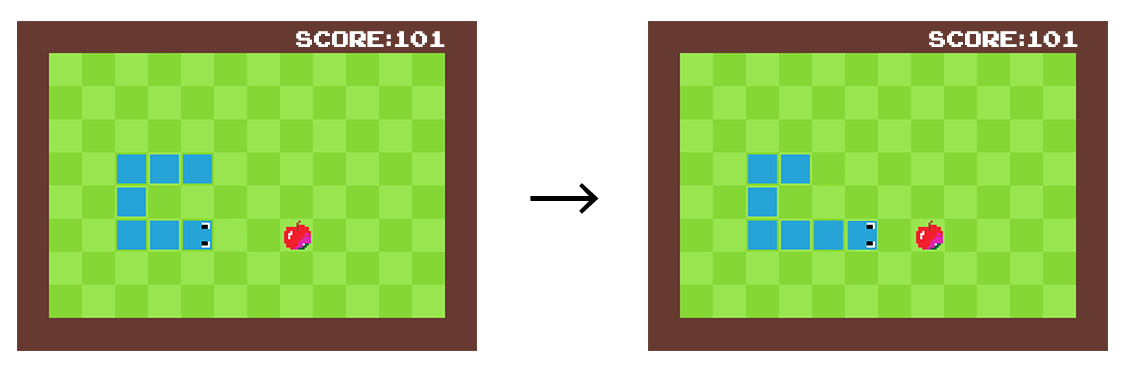
\includegraphics[width = \linewidth]{img/snake.png}
\end{center}

In this question, you will make use of the list node class `\ttt{Node}' defined below to implement several operations of the doubly-linked-list in C++ to support this game.

\begin{cpp}
    struct Node {
      int x, y;
      Node *prev, *next;
      Node(int _x, int _y, Node *_prev, Node *_next)
    	  : x(_x), y(_y), prev(_prev), next(_next) {}
    };
    Node *head, *tail;
\end{cpp}

Please pay attention to the following rules.

\begin{itemize}
	\item Use \bluett{new} and \bluett{delete} to deal with memory issues.
	\item Use \bluett{nullptr} (instead of \bluett{NULL}) for null pointer value.
	\item Make sure your code \textbf{compiles} and does not cause \textbf{runtime-errors} or \textbf{memory-leaks}.
	\item You can fill in each blank line with at most one statement. You don't have to use all of the blank lines.
	\item For simplicity, you can directly access node attributes like \ttt{node->prev}, \ttt{node->next}, etc. This is not recommended for practical programming but OK for this question.
\end{itemize}

\pagebreak

\begin{parts}
	\part[5] \textbf{Update the Snake Head}\par
	We want to create a new node to store the new location of the snake head, and insert it before the original head. You may assume that the snake has at least two nodes. Please fill in the blanks below.
	%%%%%%%%%%%%%%%%%%%%%%%%%%%%%%%%%%%%%%%%%%%%%%%%%%%%%%%%%%%%%%%%%%%%%%
	% Replace '____________' below with your code!
	%%%%%%%%%%%%%%%%%%%%%%%%%%%%%%%%%%%%%%%%%%%%%%%%%%%%%%%%%%%%%%%%%%%%%%
	\linespread{1.5}
	\begin{cpp}
void update_head(int x, int y) {
  Node *new_head = new Node(x, y, nullptr, head);
  head->prev = new_head;
  head = new_head;
}
	\end{cpp}
	\linespread{1}
	\part[5] \textbf{Remove the Snake Tail}\par
	We want to remove the tail node of the snake and update the information of the tail. You may assume that the snake has at least two nodes. Please fill in the blanks below.
	%%%%%%%%%%%%%%%%%%%%%%%%%%%%%%%%%%%%%%%%%%%%%%%%%%%%%%%%%%%%%%%%%%%%%%
	% Replace '____________' below with your code!
	%%%%%%%%%%%%%%%%%%%%%%%%%%%%%%%%%%%%%%%%%%%%%%%%%%%%%%%%%%%%%%%%%%%%%%
	\linespread{1.5}
	\begin{cpp}
void remove_tail() {
  Node *old_tail = tail;
  tail = tail->prev;
  tail->next = nullptr;
  delete old_tail;
}
	\end{cpp}
	\linespread{1}

	\part[2] \textbf{Eat the Fruit}\par
	If the snake head would touch the fruit at \((x,y)\) after a certain step, the snake will eat the fruit and increase its length by one node. Then for this step, which of the following operations should we call? Tick (\(\surd\)) the correct answer.

	%%%%%%%%%%%%%%%%%%%%%%%%%%%%%%%%%%%%%%%%%%%%%%%%%%%%%%%%%%%%%%%%%%%%%%
	% Replace `\choice' with `\CorrectChoice' on the selected choice!
	%%%%%%%%%%%%%%%%%%%%%%%%%%%%%%%%%%%%%%%%%%%%%%%%%%%%%%%%%%%%%%%%%%%%%%
	\begin{checkboxes}
		\choice \ttt{remove\_tail()}
		\CorrectChoice \ttt{update\_head(x, y)}
		\choice \ttt{update\_head(x, y)} and \ttt{remove\_tail()}
	\end{checkboxes}
\end{parts}